\documentclass[a4paper,openany,nobib]{tufte-book}

%%math stuff
\usepackage{mathtools}
\usepackage{amssymb}

%%define colours
\usepackage{xcolor}
\definecolor{tred}{HTML}{450000}
\definecolor{tgray}{HTML}{161616}

%%pictures
\usepackage{graphicx}
\graphicspath{{./pics/}}
\setkeys{Gin}{width=\linewidth}%,totalheight=\textheight,keepaspectratio}

%%pagestyle
\usepackage[protrusion=true,expansion]{microtype}
\usepackage{booktabs}
\usepackage{fancyvrb}
\usepackage{lscape}
\fvset{fontsize=\normalsize}
\fancypagestyle{plain}{}

%%questionnaire macros
\usepackage{forloop}% used for \Qrating and \Qlines
\newcommand{\Qline}[1]{\noindent\rule{#1}{0.6pt}}
\newcounter{ql}
\newcommand{\Qlines}[1]{\forloop{ql}{0}{\value{ql}<#1}{\vskip0em\Qline{\linewidth}}}

%%references
\usepackage[backend=biber,citestyle=authoryear,bibstyle=numeric,firstinits=true,autocite=footnote]{biblatex}
\addbibresource{ref.bib}
\usepackage[nottoc,notlot,notlof]{tocbibind}

%%final styling
\title{Pupil misconceptions:\\ \noindent circuits and voltage}
\author{Zella Baig}
\publisher{\today}
%\color{tgray}
%\colorlet{darkgray}{tred}
\begin{document}
%%%%
%TODO: REMOVE 100 words
%%%%
\frontmatter
{\maketitle}
\tableofcontents
\thispagestyle{empty}
\mainmatter
\chapter{Background \& Outline}
\setcounter{page}{1}
It is well established that school-age children often struggle with the concept of 'electricity'\autocite{psillos}.
This manifests in many ways;
via misconceptions regarding physical processes which occur in circuits, the mechanisms through which they occur, or through manipulations of circuitry. Much discussion has gone into examining the origins of these misconceptions,
which lead to students conceptualising 'electricity' incorrectly.
Regardless, it is known that these misconceptions are both difficult to identify, and unlearn (despite targeted education on these topics)
\autocite{lee2001}.
The aim of this report is to examine these misconceptions with both primary data collected from a local school, as well as secondary reading on the subject matter.

One concept which appears repeatedly as causing difficulty is voltage: not only is this concept fundamentally {misunderstood \autocite{shipstone_children}}, but when it \emph{does} play a part within students' reasoning for circuit theory it often plays a secondary role to other concepts (chiefly, current).
This may, perhaps, be related to the method of teaching. 
Härtel discusses how students' reasoning seems to follow the {order\autocite{hartel82}}:
\begin{align*}
	\text{Current}\rightarrow \text{Charge} \rightarrow \text{Voltage} \rightarrow \text{Resistance}
\end{align*}
which is to say that voltage is only considered \emph{after} students have examined the current and charge responses. This is, of course, problematic given how \emph{voltage} is often the initial concept \emph{causing} the various responses in the current (considering theenergy changes which occur, physically).

Before discussing the misconceptions which students hold when analysing circuits, it is worth examining the reasons \emph{why} they might hold the ideas they do.
Relevant to the previous point made about discussion of energy, many of these texts (such as Härtel, 1982) discuss how students refuse to think in terms of energy in circuits (or when they do consider it, get it confused with 'current' or 'electricity').
Another, perhaps more relevant point to this discussion, is the idea of models.

Upon learning new ideas students are likely to adopt various models to help explain these {ideas\autocite{bagno2000}}, but often encounter difficulty within circuits \& electricity to do so due to a lack of real-world links between the microscopic behaviour within the circuits to macroscopic phenomena. Students have incorrect models, misapply models, or are unable to map behaviours between models and 'actual' circuit phenomena.

As Gutwill et al. state, there is difficulty in linking ``mechanisms'' \& {``representations''\autocite{gutwill99}}.
Students usually view circuits from three different perspectives:
\begin{enumerate}
	\item Microscopic, e.g. charge carriers
	\item Aggregate, e.g. considering current and potential difference
	\item Topological, e.g. open/closed circuits and distances between components
\end{enumerate}
Bearing in mind the previous discussion (students having ill-defined ideas of various circuit phenomena outright), one may see how students would encounter difficulty in linking their physical intuitions not only to each of the perspectives individually, but also of trying to relate changes in one to those in another, given how sub-concepts are already poorly defined. More generally, it appears that students think of perturbations of circuits in three broad {models\autocite{ates2005}}:
\begin{enumerate}
	\item Sequentially, where current is affected by changes as it travels
	\item Locally, where perturbations are contained within a branch of the circuit
	\item Via superposition, where changes can be seen to be 'stacked' on top of pre-existing conditions
\end{enumerate}
When looking at the exact ``mechanisms'' employed within these models, it is worth discussing \emph{phenomenological primitives}, or \emph{p-prims} for {short\autocite{prim}}. 

P-prims (representing intuitive ideas which ``are usually evident in our everyday experience''), or their lack, may be one avenue through which these misconceptions arise. If the knowledge which students are fed is obfuscated from their own lines of reasoning - either from superfluous teaching of models when ideas may be self developed or through being taught in a manner too 'abstract' for students to pick up on at a p-prim level, students may not only pick up incorrect ideas but find it more difficult to adjust their misconceptions. 
This conclusion is backed up by Ugur et {al.\autocite{ugur}}, where it was found that misconceptions remained despite targeted teaching.

Expanding upon this, in work done by Chi \& Slotta\autocite{slotta} there is evidence to suggest that the difficulties in constructing correct models and changing incorrect ones, lie with the ontological catagorisation of the ideas involved: Lee and Law\autocite{lee2001} discuss how:
\begin{itemize}
	\item Students catagorise ideas as either 'matter' based, or 'process' based;
	\item Students seem to prefer 'matter' based models of circuits;
	\item Evidence suggests that 'process' based models provide better understanding of circuit behaviour;
	\item And perhaps most interestingly, that voltage was thought of as 'process' based more often than other circuit concepts.
\end{itemize}
What we see here links to our earlier discussion on p-prims:
in seeing concepts as 'matter' based perhaps students are employing intuitive matter-based p-prims (and extending this, may lack the necessary p-prims to conceptualise voltage in the same manner). This, along with the preference to catagorise voltage as a 'process' concept may be evidence that students have a lack of intuitive parallels for voltage than for other concepts in circuit theory - and and that teaching might need to specifically address this.

Examining the models themselves, Osborne\autocite{osb} identified several recurring misconceptions which students seemed to have, and in fact still seem to {have in modern education\autocite{suryadi2020}}:
\begin{itemize}
	\item The battery as a source of \emph{current} 
	\item Current being 'used up' by components as it travels
	\item \emph{Sequential reasoning}, where changes propagate along the flow of current
	\item \emph{Local reasoning}, where only isolated parts (e.g. a single branch) of the circuit are examined
\end{itemize}
Again, several of these misconceptions can be tied directly to a lack of conceptual understanding of the 'changes' which occur within a circuit - which itself links to the notion of voltage and what that represents in terms of energy flow; similar views have been expressed in literature such as Eylon and Ganiel\autocite{eylon1990}

Thus, this report shall focus on examining the misconceptions which students hold with the inter-relations of energy, voltage, \& current, and seek to examine the conceptual processes which students undergo when dealing with these ideas.
\newpage
\chapter{Methodology}%
The design of the surveys given to students was largely based off of those conducted in previous literature, such as by Shipstone et al., Afra et al., or Küçüközer and Kocakülah\autocite{shipstone_europe,afra2009,kucu2007}. In essence, the survey has been designed to incorporate a range of short and long-form responses, based upon circuit diagrams which are given to the students. When used, all component values were chosen that integer values would be obtained for any reasonably possible calculation such that the focus of the student remain on the conceptual ideas of the question as opposed to the mathematics.

The survey was given to two Year 9 classes and three Year 10 classes, for a total of 84 responses (split $35+49$ for each year group respectively). The Y9 group had covered electricity at a pre-GCSE level, and the Y10 group at a GCSE level. The survey was split into 3 sections:
\begin{itemize}
	\item[S1.] Series and Parallel Circuits
	\item[S2.] Circuit Ideas
	\item[S3.] Circuit Reasoning
\end{itemize}
\marginnote{Full copies of the surveys given to the pupils are available in Appendix A}
S1 dealt with steady-state behaviour and changes in both series and parallel circuits with multiple resistances. With the exception of a question asking for an explanation of any perceived differences between series and parallel circuits, all the prompts were multiple choice. This section was designed to be the most standard - almost akin to what these students would have encountered during their secondary education. The aim of this section was to identify any glaring misunderstandings of circuit behaviour and perturbations.

S2 broadly covered two topics:
that of potential difference (examining what it was thought to be and what purpose it served), and that of differences \& perturbations within circuits at a conceptual level; that is to say examining how students approach these concepts in relation to ideas such as ``charge'' or ``potential difference''. 
To this end, no numerical responses were required (though basic component values were given for clarity).

S3, the final section, was purely open ended and asked the students to compare a series and parallel configuration of bulbs in an otherwise identical configuration, and also to highlight any further difficulties with the idea of ``voltage''.
The first question in this section was deliberately left open-ended, as to be able to ascertain what links and comparisons with bulb brightness to circuit ideas could be drawn up by the students themselves - in short, this section served to draw out their self-employed methods for tackling circuit problems.
\chapter{Results}
\marginnote{The full data for responses is available in Appendix A.}
As expected, the Y10 cohort generally gave responses more in line with scientifically accepted views, though misconceptions were nevertheless common. We present a detailed breakdown by section below.
\marginnote{
In order to keep figures distinct, when percentages are given in the form 
\begin{equation*}
	(X\%, Y\%)
\end{equation*}
it is to be understood that $X\%$ of the Y9 cohort responded as such, and similarly for $Y\%$ and the Y10 cohort.}
\newthought{\LARGE{Section 1:}}

Perhaps unsurprisingly, this section highlighted several key misconceptions regarding the both the nature of voltage, as well as an interesting observation regarding Ohm's Law. 
Starting off with Q1 (question $1$), students were able to ascertain that the current would drop,
but only ($43\%,57\%$) said that it would immediately halt - perhaps suggesting a flaw in the internal models of \emph{flow} which the students employed, which would have given the charge carriers some inertia. 
On Q2, only ($11\%, 20\%$) were able to state that the potential difference across a battery remains constant, which relates to the misunderstanding of the purpose of a battery as discussed in literature\autocite{shipstone_children}. 

For Q3-Q6, the results suggest that students have a flawed understanding of Ohm's Law. Q3 was answered correctly by only ($20\%,37\%$), but more interesting are the results for Q4. $60\%$ of the Y9 cohort stated that the current through the preceding, highter ohmage resistor was \emph{higher}, but the dominant view for Y10 was that it was \emph{lower}, stated by $47\%$. It appears here that Y9 students directly related higher resistance with higher voltage, whereas Y10 can be seen as using a 'consumed current' model - a common misconception in literature.

Y9 again in Q5 link resistance and voltage incorrectly, with $69\%$ stating that the voltage across a $2\Omega$ resistor in parallel is $2V$; the modal response for Y10 suggests an incorrect application of adding resistances in parallel. 

In Q6 we see Y9 once more linking resistance directly to current, with $34\%$ stating that the current through an $8\Omega$ resistor is higher than that of a $2\Omega$ resistor; this drops to $17\%$ in Y10 but interestingly those who said it was the same remains somewhat stable at ($46\%,35\%$). Unfortunately, Q7 did not provide much insight with the few useful results simply parroting the splitting (or lack thereof) of current and voltage in series/parallel circuits.
\newpage
\newthought{\LARGE{Section 2:}}

Q8 looked at what 'potential difference' was seen to be. Reassuringly, the majority ($57\%,60\%$) were able to give a correct response in terms of energy and charge carriers. However, ($29\%,19\%$) \& ($11\%,17\%$) stated that potential difference was either a \emph{force} or a property of current - the latter again brought up in literature as a common misconception, and the former perhaps denoting a flaw in the models employed which are often matter-based.

Q9 questioned the role of a battery. For both cohorts, responses were evenly split amongst the 4 options available:
\emph{
\begin{enumerate}
	\item To act as a current source
	\item To provide energy for charge carriers
	\item To create energy as charge
	\item To act as a voltage source
\end{enumerate}}
This perhaps highlights a lack of fundamental understanding of the underpinnings of energy within circuit theory, and thus a misunderstanding of voltage (and the role thereof) follows.

Q10 \& Q11 sought to analyse sequential and continuity-based logic within circuits; they demonstrated that ($46\%,38\%$) saw current as \emph{discontinuous} within a simple series circuit, and on top of that only ($23\%,45\%$) were able to deduce that voltage across a circuit is the same as voltage across the battery, again highlighting issues with potential difference.

Reassuringly however, Q12 showed that at least on some level GCSE circuit theory was able to dispel the notion of a sequentially perturbed circuit (another commonly highlighted misconception), with ($34\%,55\%$) stating that any changes were seen immediately. Again, unfortunately Q13 was not able to discern much about their underlying ideas - though an often-cited justification for one ammeter or the other changing first was based on distance from the battery.

\newthought{\LARGE{Section 3:}}

Q14 was able to offer some further insight on the differences students saw in series and parallel circuits, with $5/23 $ responses from Y9 mentioning some physical aspect of the circuit (e.g. distance to battery) being responsible for any changes in brightness. An important note at this point is that most of the responses ($12$) were either simple statements on relative brightness, or statements of confusion - which greatly reduced the pool of valid responses.

In Y10, of 41 responses, 11 made simple references to splitting of current/voltage with explicit reference to series/parallel circuitry, with another 12 making the same statement without such references. Statements expressing thoughts such as \emph{``The current is shared''} or \emph{``The voltage is split''} were common, which demonstrates at least a basic understanding of circuit differences. However, it raises the question of how much of this is rote memorisation, and how much is truly conceptually understood.

Q15 did not give much insight, with $(79\%,35\%)$ offering no usable information. However, 3 responses of the 19 Y9 responses stated that they had not studied voltage, which would go on to explain the overall better performance of the Y10 cohort. Further, $6/23$ Y10 responses made reference to general confusion on voltage; this may suggest a need to teach this topic in even greater detail.
\chapter{Conclusion}%

The results regarding students' misconceptions with the nature of voltage are directly in line with what literature suggests - namely that it is ill-understood. The results of S1 \& S2 also demonstrated that students' internal models may be flawed - with a lack of focus on energy changes within circuits being the ultimate cause behind any subsequent phenomena, as discussed in work by Eylon and Ganiel. We see how this may credit the work done by Chi \& Slotta, demonstrating a 'matter' based approach to circuit reasoning, although this has not been verified within this study.

We also see evidence of the models proposed by Osborne, such as the current being used up and perturbations occurring sequentially. Furthermore, we also see evidence in some scenarios (such as in Q12) that further education was able to dispel these misconceptions - though it is interesting to note we see this in areas that are already well-understood to cause concern with students.

The key concerns brought up by this study seem to be:
\begin{itemize}
	\item A misunderstanding of Ohm's law
	\item Unclear links to energy within circuits
	\item Possible rote memorisation of tools rather than understanding the logic behind them
\end{itemize}
with the first point appearing repeatedly in S1 \& S2, where a higher resistance was linked to both a higher current and higher voltage across the components in question.
The second point is brought up more perhaps in the extended responses, in justifications for decisions made in earlier questions. Here we see flaws in the internal model(s) used by students; they rarely seem to incorporate the transfer and transformation of energy, and instead rely on a 'dynamic' model - again demonstrating what can be thought of as matter-based p-prims.
\marginnote{This dynamical preference illustrated well, for example, by one student who stated that an ammeter would \emph{``notice the change of resistance before [the other ammeter]''}}
Lastly, an issue which might be difficult to pick up in the classroom is the third point raised: the justifications given for reasoning often seem to imply that students are parroting facts about what circuits behave like,
as opposed to understanding why it is that a given phenomena occurs, best demonstrated in the questions where students were asked to justify reasoning: many simply stated that circuits were series/parallel.

These areas as well as the other well-established misconceptions regarding voltage should be both investigated and targeted within the classroom. It appears that there is a gap in the existing models with regards to both the inclusion of energy to an appropriate degree, as well as a lack of focus on voltage, which leads to poor understanding and incorporation of these concepts within reasoning. Further, it appears that Ohm's law is one tool where students perform poorly (being unable to manipulate the equation conceptually, without values) and that this may tie into the previous point: Ohm's law may be fundamentally misunderstood or difficult to conceptualise.
Importantly, the current form of education must seek to move away from encouraging memorisation of facts and instead towards understanding why they hold; energy would naturally appear here more frequently given its fundamental role in much of physics and so perhaps a shift in teaching away from focusing on the \emph{dynamical} aspects of models to the \emph{energy} aspects is required as to instill these concepts fully. For example, in teaching circuits using a waterfall model, linking more strongly the GPE water has at the top to the energy given by the battery, and explaining the splitting of voltage/current in series/parallel through the usage of turbines in the water stream arranged in series/parallel alongside potential energy changes. Care must be taken not to link these ideas too strongly to everyday dynamical models (or rather, to make it clear how said models can be overextended).
Further, this does present the difficulty in forming links to well-established phenomena in students' lives: further investigation is needed as to the exact nature of the links between circuits and everyday occurrences.

Ultimately, while the study was performed only at one school using a single method of teaching, there was clear improvement over the 2 year groups examined; this is a positive outcome as it suggests that further targeted education on these specific areas may seek to reduce these misconceptions further; with further study we should be able to narrow down the sources of misconceptions and help prevent them from forming.
\backmatter
\chapter{Appendix A: Questionnaire}
\marginnote{This section contains a remake of the questionnaire, sent initially on Google Forms, and as such is formatted slightly differently to the one sent to students. All content remains the same

A read-only copy of the questionnaire is viewable at: \href{https://forms.gle/d9x5bSBppvJrQ4aA9}{https://forms.gle/d9x5bSBppvJrQ4aA9}}
The goal of this questionnaire is, to put it briefly, to analyse how students think about circuits and energy, as well as related ideas. The goal isn't to get all the answers right - indeed for some of the questions there are no right answers at all (though there are for others - which you should try to answer to the best of your ability). Instead, the questions will try to focus on understanding how you might go about thinking about circuits, and how you apply those ideas to questions you encounter.

The information gathered from these responses will be used as part of a wider report on the difficulties and misconceptions students have with circuit ideas - in particular the nature and role of voltage, which has generally been known to cause more issues than other concepts within circuit.

\marginnote{Though the questions were not numbered as such, tables shall be given as follows:}
\begin{margintable}
  \begin{center}
    \begin{tabular}{crr}
      \toprule
      Choice: & Y9: & Y10:\\
      i & 2 & 5 \\
      ii & 12 & 10\\
      iii & 5 & 15\\
      iv & 1 & 5\\
      \bottomrule
    \end{tabular}
	\caption{\centering Q1}
  \end{center}
\end{margintable}
\marginnote{with the choices i-iv representing the multiple choice options, and $Q_n$ representing the $n^{th}$ question.}
When desired, you may refer to figures and components by the abbreviations given (for example, shortening Circuit 6 to C6); note however this is not mandatory.

Responses will be anonymised within the report.

\newthought{\LARGE{A refresher}}

As you may recall from your classes, circuits involve several conceptual ideas such as voltage (measured in volts), current (measured in amperes), power (in watts), charge (in coulombs), and energy (in joules) - amongst many others. 

To give a brief overview, some energy source (usually a battery) enables the flow of charge within a circuit (usually through electrons in wires), which allows the circuit to 'do' things, such as powering a bulb, turn on a screen, or many other things. This section will get you to analyse this idea in more detail, as well as perform some calculations with some example circuits.

You may also remember that there are 2 broad types of circuits - series (such as Circuit 2, which you will encounter below) and parallel (such as Circuit 3). These types behave in different ways - and part of the questions will try to look at how you think about their differences and similarities in your head.
\newpage
\newthought{\LARGE{Section 1}}
\begin{figure}[h!]
	\center
	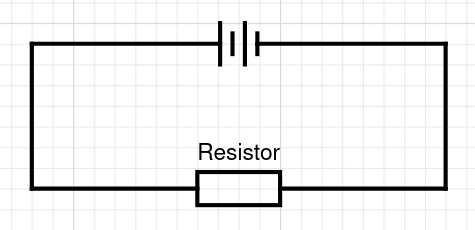
\includegraphics[width=\linewidth]{simple}
	\caption[][2cm]{Circuit 1}
	\label{fig:marginfig}
\end{figure}
\begin{enumerate}
    \item What would happen to the reading on a voltmeter connected across the resistor if I disconnect the battery from the circuit?

		\begin{margintable}[1cm]
  \begin{center}
    \begin{tabular}{crr}
      \toprule
      Choice: & Y9: & Y10:\\
      i & 15 & 28\\
      ii & 19 & 16\\
      iii & 1 & 5\\
      iv & 0 & 0\\
      \bottomrule
    \end{tabular}
	\caption{\centering Q1}
  \end{center}
\end{margintable}

		\begin{itemize}
\item[$\square$]It would immediately drop to $0$ V
	\item[$\square$]It would slowly drop to $0$ V
	\item[$\square$]It would stay the same
		\item[$\square$]It would rise to infinity
\end{itemize}
\item Now, what would happen to the voltmeter reading across the battery if I disconnect the battery from the circuit?
	\begin{margintable}
	\begin{center}
	\begin{tabular}{crr}
	\toprule
	 Choice: & Y9: & Y10:\\
	 i & 20 & 32\\
	 ii & 11 & 7\\
	 iii & 4 & 10\\
	 iv & 0 & 0\\
	 \bottomrule
	\end{tabular}
	\caption{\centering Q2}
	\end{center}
	\end{margintable}
	\begin{itemize}
\item[$\square$]It would immediately drop to $0$ V
	\item[$\square$]It would slowly drop to $0$ V
	\item[$\square$]It would stay the same
		\item[$\square$]It would rise to infinity
	\end{itemize}
\end{enumerate}
\begin{figure}[h!]
	\center
	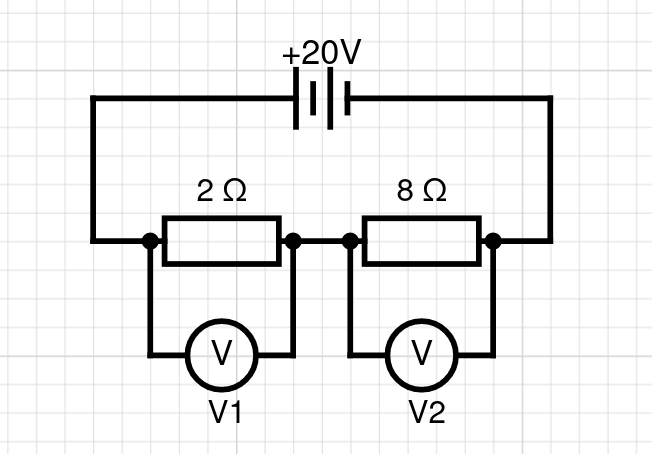
\includegraphics[width=\linewidth]{circ2}
	\caption[][2cm]{Circuit 2}
\end{figure}
\newpage
\begin{enumerate}
	\setcounter{enumi}{2}
	\item In Circuit 2, what is the reading on voltmeter V2 (which measures the potential difference across the 8 ohm resistor). 
		\begin{margintable}
		\begin{center}
		\begin{tabular}{crr}
		\toprule
		 Choice: & Y9: & Y10:\\
		 i & 7 & 18\\
		 ii & 5 & 11\\
		 iii & 4 & 7\\
		 iv & 19 & 13\\
		 \bottomrule
		\end{tabular}
		\caption{\centering Q3}
		\end{center}
		\end{margintable}
		\begin{itemize}
			\item[$\square$]$16$ V
			\item[$\square$]$4$ V
			\item[$\square$]$2$ V
			\item[$\square$]$8$ V
		\end{itemize}
	\item Compared to the 2 ohm resistor, the current going through the 8 ohm resistor is...
		\begin{margintable}[1cm]
		\begin{center}
		\begin{tabular}{crr}
		\toprule
		 Choice: & Y9: & Y10:\\
		 i & 8 & 12\\
		 ii & 6 & 22\\
		 iii & 21 & 13\\
		 \bottomrule
		\end{tabular}
		\caption{\centering Q4}
		\end{center}
		\end{margintable}
	\begin{itemize}
		\item[$\square$] The same
		\item[$\square$] Lower
		\item[$\square$] Higher
	\end{itemize}
\end{enumerate}
\begin{figure}[h!]
	\center
	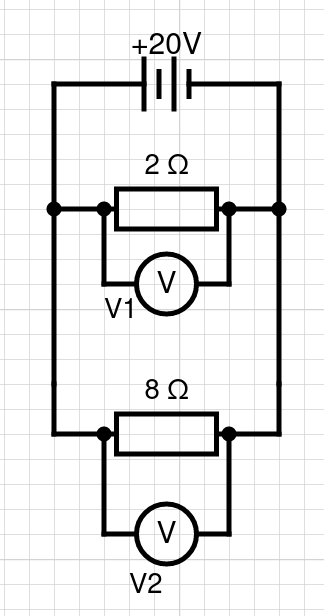
\includegraphics[width=0.5\linewidth]{circ3}
	\caption[][3cm]{Circuit 3}
\end{figure}
\begin{enumerate}
		\newpage
	\setcounter{enumi}{4}
	\item In Circuit 3, what is the voltmeter reading for V1:
		\begin{margintable}
		\begin{center}
		\begin{tabular}{crr}
		\toprule
		 Choice: & Y9: & Y10:\\
		 i & 5 & 24\\
		 ii & 24 & 8\\
		 iii & 6 & 16\\
		 iv & 0 & 1\\
		 \bottomrule
		\end{tabular}
		\caption{\centering Q5}
		\end{center}
		\end{margintable}
		\begin{itemize}
			\item[$\square$]$10$ V
			\item[$\square$]$2$ V
			\item[$\square$]$20$ V
			\item[$\square$]$2.5$ V
		\end{itemize}
	\item Compared to the 2 ohm resistor, the current going through the 8 ohm resistor is...
		\begin{margintable}[1cm]
		\begin{center}
		\begin{tabular}{crr}
		\toprule
		 Choice: & Y9: & Y10:\\
		 i & 16 & 17\\
		 ii & 7 & 23\\
		 iii & 12 & 8\\
		 \bottomrule
		\end{tabular}
		\caption{\centering Q6}
		\end{center}
		\end{margintable}
	\begin{itemize}
		\item[$\square$] The same
		\item[$\square$] Lower
		\item[$\square$] Higher
	\end{itemize}
\item For the questions before on Circuits 2 and 3, explain the differences in your answer, if any. Answer in terms of energy, charge, voltage, and current.
	\marginnote{Of 25 responses from Y10, 16 were simple statements about the circuits being either series or parallel, 8 offered no insight, and 1 made reference to energy. Of 17 responses from Y9, 14 expressed confusion (perhaps suggesting this question was pitched too high).}
		\Qlines{2}
\end{enumerate}
\newpage
\newthought{\LARGE{Section 2}}
\begin{enumerate}
	\setcounter{enumi}{7}
		\item What is potential difference? Do not answer in terms of formulae, instead think about what what this term represents in terms of charge.
			\begin{margintable}
			\begin{center}
			\begin{tabular}{crr}
			\toprule
			 Choice: & Y9: & Y10:\\
			 i & 4 & 8\\
			 ii & 20 & 29\\
			 iii & 10 & 9\\
			 iv & 1 & 2\\
			 \bottomrule
			\end{tabular}
			\caption{\centering Q8}
			\end{center}
			\end{margintable}
			\begin{itemize}
				\item[$\square$]A property of current which relates it to the energy carried by the charge carriers
				\item[$\square$]The difference in energy between 2 points through which charge carriers travel
				\item[$\square$]The force that acts on the charge carriers between 2 points in a circuit
				\item[$\square$]The force caused by the charge carriers between 2 points on a circuit
			\end{itemize}
		\item What is the role of a battery in a circuit?
			\begin{margintable}[2cm]
			\begin{center}
			\begin{tabular}{crr}
			\toprule
			 Choice: & Y9: & Y10:\\
			 i & 9 & 13\\
			 ii & 8 & 14\\
			 iii & 8 & 11\\
			 iv & 10 & 11\\
			 \bottomrule
			\end{tabular}
			\caption{\centering Q9}
			\end{center}
			\end{margintable}
		\begin{itemize}
			\item[$\square$]To act as a source of current
			\item[$\square$]To provide energy to the charge carriers
			\item[$\square$]To create energy in the form of charge
			\item[$\square$]To act a source of voltage
		\end{itemize}
\end{enumerate}
\begin{figure}[h!]
	\center
	\includegraphics[width=\linewidth]{Vary}
	\caption[][3cm]{Circuit 4}
\end{figure}
\begin{enumerate}
		\setcounter{enumi}{9}
		\item Consider Circuit 4. The readings on the ammeters (which measure the current going through them) AM1 and AM2 are:
			\begin{margintable}
			\begin{center}
			\begin{tabular}{crr}
			\toprule
			 Choice: & Y9: & Y10:\\
			 i & 19 & 30\\
			 ii & 16 & 18\\
			 \bottomrule
			\end{tabular}
			\caption{\centering Q10}
			\end{center}
			\end{margintable}
		\begin{itemize}
			\item[$\square$] The same
			\item[$\square$] Different
		\end{itemize}
	\item The readings on the voltmeters VM1 and VM2 are:
		\begin{margintable}[0cm]
		\begin{center}
		\begin{tabular}{crr}
		\toprule
		 Choice: & Y9: & Y10:\\
		 i & 8 & 22\\
		 ii & 27 & 27\\
		 \bottomrule
		\end{tabular}
		\caption{\centering Q11}
		\end{center}
		\end{margintable}
		\begin{itemize}
			\item[$\square$] The same
			\item[$\square$] Different
		\end{itemize}
	\item Consider Circuit 4 in terms of the flow of charge, and what is going on with the charge carriers. Suddenly, I change the resistance of the resistor. What is the correct ordering of events?
		\begin{margintable}
		\begin{center}
		\begin{tabular}{crr}
		\toprule
		 Choice: & Y9: & Y10:\\
		 i & 11 & 11\\
		 ii & 11 & 7\\
		 iii & 12 & 26\\
		 iv & 1 & 3\\
		 \bottomrule
		\end{tabular}
		\caption{\centering Q12}
		\end{center}
		\end{margintable}
		\begin{itemize}
			\item[$\square$] AM1 changes, then AM2 does
			\item[$\square$] AM2 changes, then AM1 does
			\item[$\square$] They both change at the same time
			\item[$\square$] Neither changes
		\end{itemize}
\item For whichever answer you chose to the previous question, explain your answer:
	\marginnote{For the 22 Y9 responses, 9 made reference to the physical position of the components, and 10 either expressed confusion or offered no insight. Of the 28 Y10 responses, 12 offered no insight, 8 made reference to the physical location, and 8 referenced conservation of charge or current.}
		\Qlines{2}
\end{enumerate}
\newpage
\newthought{\LARGE{Section 3}}
\begin{figure}[h!]
	\center
	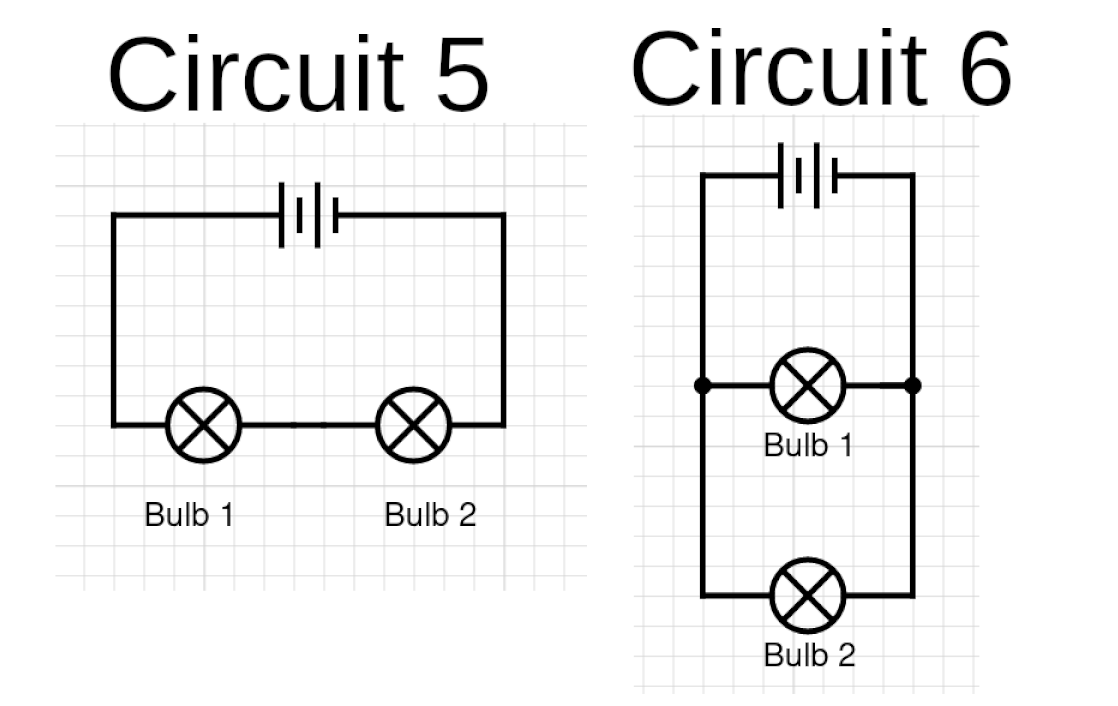
\includegraphics[width=\linewidth]{comp}
	\caption[][3cm]{Circuits 5 \& 6}
\end{figure}
\begin{enumerate}
		\setcounter{enumi}{13}
		\marginnote[-1.5cm]{For the 23 Y9 responses, 12 were simple statements on brightness or confusion, 5 were on physical aspects of the circuit, 4 made reference to energy in the justification, and 2 were on the sharing of voltage. Of the 41 Y10 responses, 11 referenced series/parallel circuits as well as splitting current or voltage, with 12 referencing splitting of current or vooltage. 2 made reference to energy within the components, 10 were simple statements on relative brightnesses, and 6 offered no insight at all.}
		\item Compare the brightness of Bulb 1 (B1) \& Bulb 2 (B2) in Circuits 5 (C5) \& Circuit 6 (C6). Assume the voltage of the battery is the same in both cases. Justify your reasoning 
		\Qlines{2}
		\item What conceptual difficulties do you have with the concept of voltage, if any?
			\marginnote[0cm]{For the 19 Y9 responses, 15 offered no insight. 1 expressed confusion on series/parallel rules, and 3 in fact stated that they had not studied this concept - which would serve to explain the overall improvements by Y10 in the questionnaire. Of the 23 Y10 responses, 4 referenced confusion over series/parallel circuits, 2 were on difficulties about experimentation using voltmeters, 3 were on the relationship between resistance and voltage, 6 were general statements on confusion regarding voltage as a concept, and 8 offered no insight.}
		\Qlines{2}
\end{enumerate}
\nocite{*}
\printbibliography[heading=bibintoc]
\end{document}
